\section{A brief primer on information theory}

\mode<presentation>{
\begin{frame} 
    \begin{center} \huge
        \secname
    \end{center}
    \begin{center}
    Key measures from information theory which play a role in formulating an optimization objective for Infomax ICA
    \end{center}
\end{frame}
}

\notesonly{
Here we go over several measures from information theory which play a role in formulating an optimization objective for Infomax ICA
}

\subsection{Entropy}

\begin{frame}{\subsecname}

Entropy is a measure of uncertainty. It measures the average amount of information conveyed by a message.

\pause

\slidesonly{

\svspace{3mm}

\begin{minipage}{.99\textwidth}
\begin{minipage}{0.3\textwidth}
	\begin{center}
		
\includegraphics[width=0.9\textwidth]{img/meme_entropy1}
	\end{center}
\end{minipage}
\hfill
\begin{minipage}{0.3\textwidth}
	\begin{center}
		
\includegraphics[width=0.7\textwidth]{img/meme_entropy2}
	\end{center}
\end{minipage}
\hfill
\begin{minipage}{0.3\textwidth}
	\begin{center}
		
\includegraphics[width=0.8\textwidth]{img/meme_entropy_none}
	\end{center}
	\end{minipage}
\end{minipage}
}

\end{frame}

\begin{frame}

\begin{block}{Entropy} 
The entropy $H(X)$ of a discrete random variable $X$ is defined by:

\begin{equation}
\label{eq:entropy}
H(X) := - \sum_{x \in \mathcal X} p_X(x)\,\log p_X(x)
\end{equation}

\end{block}

Imagine flipping a biased coin which reveals \textit{tails} most of the time. 
We will no longer be ``surprised'', if we flip the coin again and see it show \textit{tails} \textbf{again}.\\

There is no information gained from flipping the coin another time. There is no uncertainty left.

However, if it were an unbiased coin, we would be equally uncertain of the outcome every time.

\end{frame}

\begin{frame}{Entropy for continuous variables}

We do not have an equivalent measure for continuous random variables. 
However we can resort to the \emph{differential entropy} $h(X)$ of a \textbf{continuous} variable $X$
\footnote{if interested, \citealp[see][Ch~10.2]{haykin1994neural} for the relation between $H(X)$ and $h(X)$.}:

\begin{equation}
\label{eq:entropydiff}
h(X) := - \int_{-\infty}^{\infty} p_X(x)\,\log p_X(x) \, dx 
= - \E \lbrack \log p_X(x) \rbrack
\end{equation}

\end{frame}

%\exercise{Joint Entropy}

%\textbf{Definition:} 
%The joint entropy of $H(X,Y)$ of a pair of discrete random variables $(X,Y)$ with a joint pdf $p_{X,Y}(x,y)$ is defined as:

%\begin{equation}
%\label{eq:entropyjoint}
%H(X,Y) = - \sum_{x \in \mathcal X} \sum_{y \in \mathcal{Y}} p_{X,Y}(x,y)\,\log p_{X,Y}(x,y)
%\end{equation}

\subsection{Conditional Entropy}

\begin{frame}{\subsecname}

Conditional entropy measures entropy of a random variable \textbf{after} one has observed the event of another variable.

\end{frame}

\begin{frame}{\subsecname}

In the case of a system with input $X$ and output $Y$.\\

\svspace{3mm}

\textbf{Definition:} 
The conditional entropy of $H(Y|X)$ of a pair of discrete random variables $(X,Y)$ with a joint pdf $p_{X,Y}(x,y)$ is defined as:

\begin{equation}
\label{eq:entropycond}
H(Y|X) = -\sum_{x \in \mathcal{X}} \sum_{y \in \mathcal{Y}} p_{X,Y}(x,y)\,\log \frac{p_{X,Y}(x,y)}{p_X(x)}
\end{equation}

\question{Where does the definition come from?}

\end{frame}

\begin{frame}{\subsecname: deriving its definition}

\begin{align}
%\label{eq:entropycond}
H(Y|X) 
&= \sum_{x \in \mathcal{X}} p_X(x) H(Y|X=x) \\
&= -\sum_{x \in \mathcal{X}} p_X(x) \sum_{y \in \mathcal{Y}} p(y|x)\,\log p(y|x) \\
&= -\sum_{x \in \mathcal{X}} \sum_{y \in \mathcal{Y}} p_X(x) p(y|x)\,\log p(y|x) \\
&= -\sum_{x \in \mathcal{X}} \sum_{y \in \mathcal{Y}} p_{X,Y}(x,y)\,\log p(y|x) \\
&= -\sum_{x \in \mathcal{X}} \sum_{y \in \mathcal{Y}} p_{X,Y}(x,y)\,\log \frac{p_{X,Y}(x,y)}{p_X(x)} \\
&= -\E_{p_{X,Y}(x,y)} \lbrack \, \log p(Y|X) \, \rbrack
\end{align}

\end{frame}

\begin{frame}{\subsecname}

\question{What does conditional entropy tell us?}

-$H(Y|X)$ represents the amount of uncertainty remaining about a system's output $Y$ \textbf{after} the 
system's input $X$ has been observed.

\pause

\question{What does this mean?} 

\pause

\emph{
$H(Y|X)$ is whatever entropy the output $Y$ has that did not come from the input $X$
}
\only<3>{
\footnote{\cite{bell1995information}}
}.

\question{And what does that mean?}


\end{frame}

\begin{frame}{\subsecname}

\slidesonly{
\emph{
$H(Y|X)$ is whatever entropy the output $Y$ has that did not come from the input $X$
} - \citeauthor{bell1995information}
}

\pause

%\svspace{-5mm}
\begin{center}
\slidesonly{
	\includegraphics<2>[width=0.55\textwidth]{img/aldisain_Plasma_TV}
	\includegraphics<3>[width=0.35\textwidth]{img/Wooden-TV_off}
	\includegraphics<4>[width=0.35\textwidth]{img/Wooden-TV_on}
	\includegraphics<5>[width=0.35\textwidth]{img/Wooden-TV_noise}
}
	\includegraphics<6,8>[width=0.35\textwidth]{img/Wooden-TV_on}
	\includegraphics<7,8>[width=0.35\textwidth]{img/Wooden-TV_noise}
\end{center}

\pause

\svspace{-3mm}

\visible<8>{

\question{Do $X$ and $Y$ have to have an input-output relationship to talk about conditional entropy?}

\notesonly{- No, this is not necessary. An input-output relationship is just a clear and intuitive way to describe dependency between the two variables.}

}

\end{frame}

\begin{frame}{\subsecname}

\slidesonly{
Same as with entropy
\svspace{5mm}
}

For the continuous case, we measure the conditional differential entropy $h(Y|X)$ which is defined as:

\begin{equation}
h(Y|X) = -\int_{-\infty}^{\infty} \int_{-\infty}^{\infty} p_{X,Y}(x,y)\,\log  p_{Y}(y|x) \, dx \, dy
\label{eq:diffentropycondcontinuous}
\end{equation}

\end{frame}

\subsection{Relative Entropy or Kullback-Leibler (KL) divergence}

\begin{frame}{\subsecname}

A measure for how much one probability distribution differs from a reference distribution. 

\textbf{Definition:} 
The relative entropy or Kullback-Leibler divergence between two pdfs $p(x)$ and $q(x)$ is defined as

%\begin{align}
%\label{eq:kldiscrete}
%D_{KL}(p||q) 
%&= \sum{x \in } p_X(x) \log \frac{p_X(x)}{q(x)} \\
%&= -\E_{p_{X}(x)} \,\log \frac{p(X)}{q(X)}
%\end{align}

%for the discrete case. And

\begin{align}
\label{eq:klcont}
\dkl\lbrack\,p\, ||\, q\,\rbrack 
&= \int_{-\infty}^{\infty} p(x) \log \left( \frac{p(x)}{q(x)} \right) dx
\end{align}

for the continuous case.

\end{frame}

\begin{frame}{\subsecname}

\begin{center}
	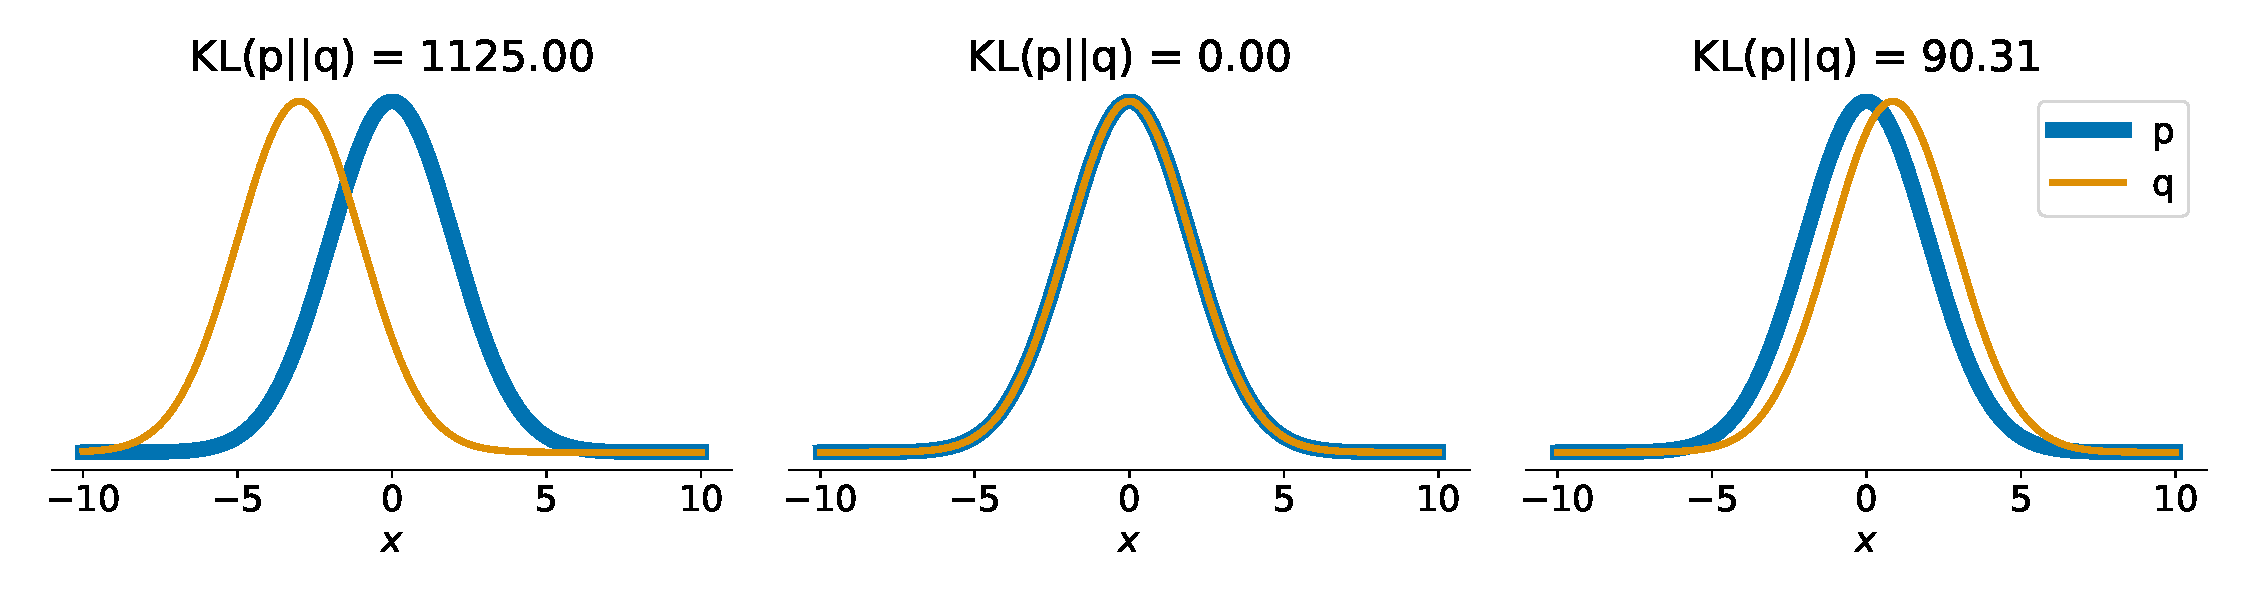
\includegraphics[width=0.8\textwidth]{img/kl_normal}
	
	\pause
	
	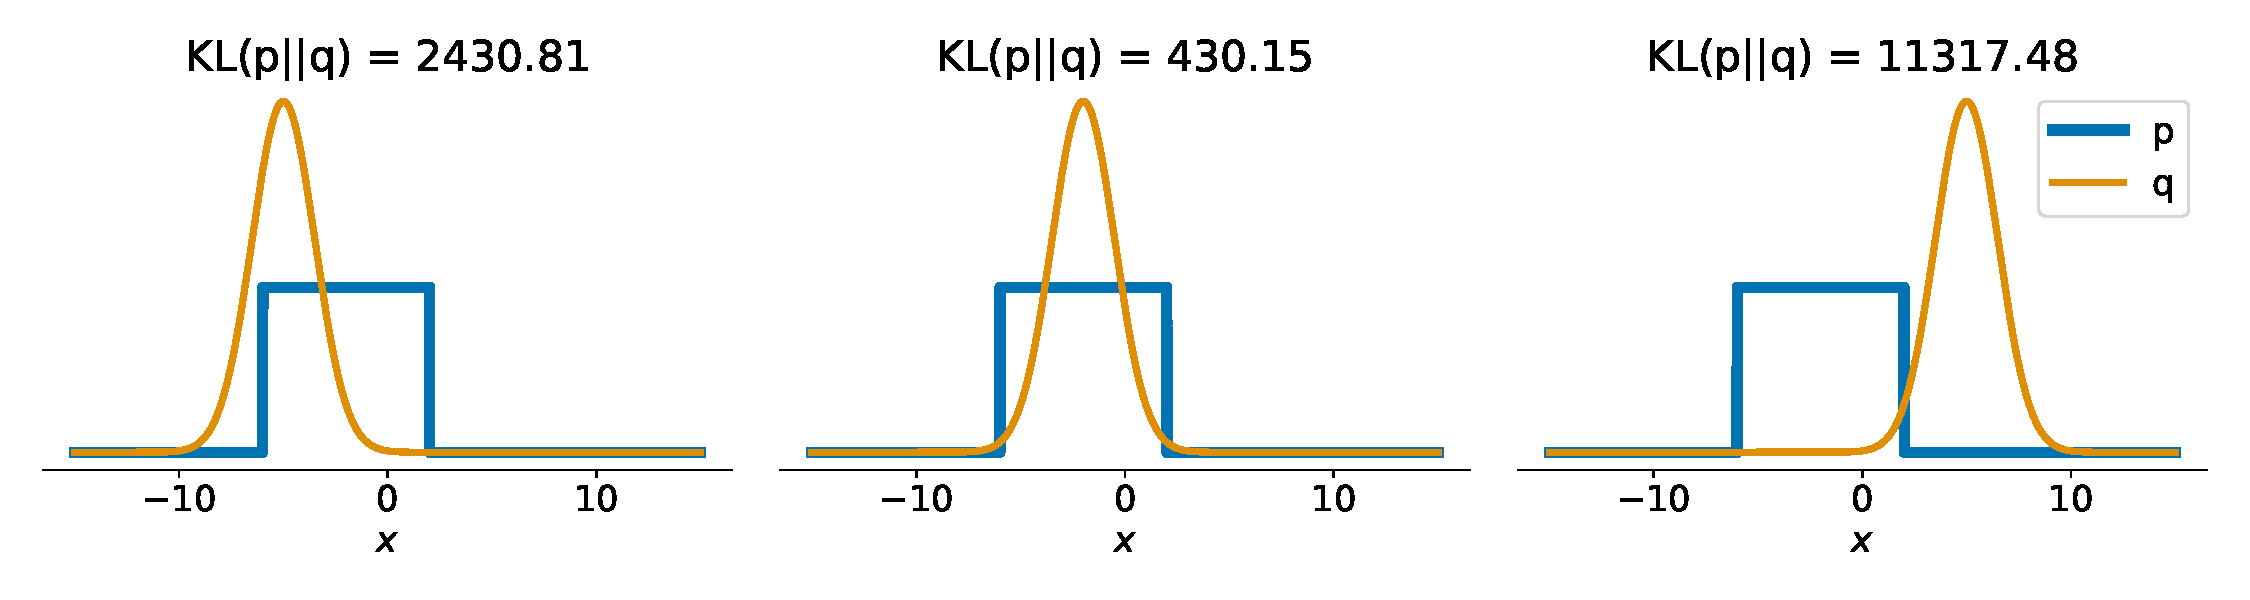
\includegraphics[width=0.8\textwidth]{img/kl_uniform_normal}
	\notesonly{
	\captionof{figure}{Measure the KL divergence between two pdfs.}
	}
\end{center}

\pause 

The KL divergence does not qualify as a distance metric, as it is not symmetric, but it still satisfies other useful metric properties:
\begin{enumerate}
\item non-negative
\item $D_{KL}\lbrack\,p\, ||\, q\,\rbrack = 0$ iff. $p = q$.
\end{enumerate}


\end{frame}


\clearpage 

\begin{frame}{Putting things into the context of ICA}
\notesonly{Let's start putting things into the context of ICA:}

\slidesonly{
\begin{center}
	
\includegraphics[width=0.6\textwidth]{img/meme_puzzle2}
\end{center}
}

\end{frame}

\begin{frame}{Putting things into the context of ICA}
\only<1>{

\slidesonly{
$$
\widehat{\vec {s}} = \vec W \cdot \vec x
$$
}

Recalling the factorization \notesonly{in \eqref{eq:facts} which is based on the assumption that }\slidesonly{\begin{equation}
%\label{eq:facts}
\widehat{P}_{\vec s}(\widehat{\vec s}) = \prod_{i=1}^{N} \widehat{P}_{s_i}(\widehat{s_i})  \,.
\end{equation}}

\notesonly{We want to }\slidesonly{$\Rightarrow$ }formulate an objective for ICA which targets our prior assumption \slidesonly{of independence}\notesonly{that the individual sources are independent from one another.}

\notesonly{The KL-divergence gives us a measure for comparing two distributions. Therefore, we can formulate the objective as }the KL divergence between the joint distribution of the sources and the product of the marginals, specifically:
}
\only<1->{
\begin{equation}
\label{eq:klmin}
	\dkl\lbrack P_{\vec{s}}(\widehat{\vec{s}}),\widehat{P}_{\vec{s}}(\widehat{\vec{s}})\rbrack = 
    \int d \, \widehat{\vec{s}} \; P_{\vec{s}}(\widehat{\vec{s}})
		\ln \frac{P_{\vec{s}}(\widehat{\vec{s}})}{
			\prod_{i = 1}^N \widehat{P}_{s_i}(\widehat{s}_i) }
		\eqexcl \min_{\vec{W}}
\end{equation}
}
\only<2->{

In spite of this being a justified approach for blind source separation, it requires a parametrized density estimate which would make this approach computationally costly.
}
\only<3>{
\slidesonly{
\begin{center}
	
\includegraphics[width=0.35\textwidth]{img/meme_anotherway}
\end{center}
}

} 
\end{frame}

\subsection{Mutual Information}

\begin{frame}{\subsecname}

\begin{itemize}
\item (differential) entropy $h(X)$ represents our uncertainty about $X$ 
and 
\item the conditional (differential) entropy $h(X|Y)$ represents such \textbf{after} observing $Y$.
\end{itemize}

Therefore, the \textbf{difference} between them represents the uncertainty about $X$ \textbf{that is resolved} after observing $Y$,

\pause

which gives us the \emph{mutual information} $I(X,Y)$ between the random variables $X$ and $Y$:

\begin{equation}
I(X,Y) = h(X) - h(X|Y)
\end{equation}

for the continuous case.

\end{frame}

\begin{frame}{\subsecname}

Properties of mutual information:

\begin{align}
\label{eq:mutualcontprops}
I(X,Y) &= h(X) - h(X|Y)\\
&= h(Y) - h(Y|X)\\
%&= h(X) + h(Y) - h(X,Y) \\
&= I(Y,X) \\
&\ge 0
\end{align}

\end{frame}

\subsubsection{Further interpretation for the mutual information}

\begin{frame}{\subsubsecname}

%\begin{align}
%\label{eq:mutualdiscrete}
%I(X,Y) &= H(X) - H(X|Y) \\
%&= \sum{x \in } \sum{y \in } p_{X,Y}(x,y) \, \log \left(\frac{p(x,y)}{p_X(x) p_Y(y)}\right)
%&= H(Y) - H(Y|X) = I(Y,X)
%\end{align}

%for the discrete case. And
\notesonly{Substituting the definitions for $h(X)$ and $h(X|Y)$:}

\begin{align}
\label{eq:mutualcont1}
I(X,Y) 
&= \int_{-\infty}^{\infty} \int_{-\infty}^{\infty} p_{X,Y}(x,y) \, \log \left(\frac{p_X(x|y)}{p_X(x)}\right) dx \, dy \\
\end{align}

\pause

and with the \emph{product rule} $p_{X,Y} = p_X(x|y)\,p_Y(y)$ we get:

\begin{align}
\label{eq:mutualcont2}
I(X,Y)
&= \int_{-\infty}^{\infty} \int_{-\infty}^{\infty} p_{X,Y}(x,y) \, \log \left(\frac{p_{X,Y}(x,y)}{p_X(x) p_Y(y)}\right) dx \, dy
\end{align}

for the continuous case.

\end{frame}




\newpage

\subsection{Relationship between the KL-Divergence and Mutual Information}

\begin{frame}{\subsecname}



This is just to show how to arrive at the same optimization problem\notesonly{ as in \eqref{eq:klmin}} through mutual information.

Recall\notesonly{ the definition of the mutual information between two variables \eqref{eq:mutualcont2}:}

\begin{equation*}
I(X,Y) = \int_{-\infty}^{\infty} \int_{-\infty}^{\infty} {\color{blue}p_{X,Y}(x,y)} \, \log \left(\frac{{\color{blue}p_{X,Y}(x,y)}}{{\color{red}p_X(x) p_Y(y)}}\right) dx \, dy
\end{equation*}

\notesonly{and the definition for the KL divergence from \eqref{eq:klcont}}

\slidesonly{
\begin{align*}
\dkl\lbrack\,p\, ||\, q\,\rbrack 
&= \int_{-\infty}^{\infty} p(x) \log \left( \frac{p(x)}{q(x)} \right) dx.
\end{align*}
}

\pause

We can deduce that:
\begin{equation}
I(X,Y) = D_{KL} \lbrack \, {\color{blue}p_{X,Y}(x,y)} \, || \, {\color{red}p_X(x) p_Y(y)} \, \rbrack
\end{equation}

\end{frame}

\begin{frame}{\subsecname}

\slidesonly{
\begin{equation}
I(X,Y) = D_{KL} \lbrack \, {\color{blue}p_{X,Y}(x,y)} \, || \, {\color{red}p_X(x) p_Y(y)} \, \rbrack
\end{equation}
}

Although $I(X,Y) = I(Y,X)$ the same cannot be said about switching the arguments of the KL-divergence.

\begin{equation}
D_{KL} \lbrack \, {\color{blue}p_{X,Y}(x,y)} \, || \, {\color{red}p_X(x) p_Y(y)} \, \rbrack \ne 
D_{KL} \lbrack \, {\color{red}p_X(x) p_Y(y)} \, || \, {\color{blue}p_{X,Y}(x,y)}\, \rbrack
\end{equation}

The above is only equal if both of them are equal to zero, which is satisfied if $p_{X,Y}(x,y) = p_X(x) p_Y(y)$.

\notesonly{
This tells us that the mutual information $I(X,Y)$ is equivalent to the KL-divergence between the joint distribution $p_{X,Y}(x,y)$ and 
the product of the pdfs $p_X(x)$ and $p_Y(y)$. A special case of this is what we saw in the first approach, namely the KL-divergence 
between the pdf of a random vector $\widehat {\vec s}$ of length $N$ and the marginal probability density functions for $N$ elements 
$\widehat{s_i}$\footnote{A much smoother walkthrough for this can be found in 
Haykin Ch. 10.5}
}
\slidesonly{
Takeaway:\\
\begin{equation}
\label{eq:klmin}
	\dkl\lbrack{\color{blue}P_{\vec{s}}(\widehat{\vec{s}})},{\color{red}\widehat{P}_{\vec{s}}(\widehat{\vec{s}})}\rbrack = 
    \int d \, \widehat{\vec{s}} \; {\color{blue}P_{\vec{s}}(\widehat{\vec{s}})}
		\ln \frac{{\color{blue}P_{\vec{s}}(\widehat{\vec{s}})}}{
			{\color{red}
			\prod_{i = 1}^N \widehat{P}_{s_i}(\widehat{s}_i) 
			}
			}
		\eqexcl \min_{\vec{W}}
\end{equation}
has an equivalent optimization in terms of mutual information.
}

\end{frame}

